\documentclass[12pt]{exam}
\usepackage{amsthm}
\usepackage{bm}
\usepackage{libertine}
\usepackage[utf8]{inputenc}
\usepackage[margin=0.5in]{geometry}
\usepackage{amsmath,amssymb}
\usepackage{multicol}
\usepackage[shortlabels]{enumitem}
\usepackage{siunitx}
\usepackage{physics}
\usepackage{booktabs}
\usepackage{graphicx}
\usepackage{pgfplots}
\usepackage{listings}
\usepackage{tikz}
\usepackage{tikz-3dplot}
\usetikzlibrary{arrows.meta,decorations.markings}

\bmdefine{\ii}{i}
\bmdefine{\jj}{j}
\bmdefine{\kk}{k}
\newcommand{\te}{\theta}
\newcommand{\cC}{\mathcal{C}}
\newcommand{\word}[1]{\quad\text{#1}\quad}

\pgfplotsset{width=10cm,compat=1.9}
\usepgfplotslibrary{external}
\tikzexternalize
\tikzexternaldisable

\newcommand{\class}{Math 261-001}
\newcommand{\examnum}{Quiz 9 Solutions}
\newcommand{\examdate}{November 6}

\begin{document}
\pagestyle{plain}
\thispagestyle{empty}

\noindent
\textbf{\class}\\
\textbf{\examnum}, \textbf{\examdate}

\vspace{8pt}
\small
\setlength{\abovedisplayskip}{6pt}
\setlength{\belowdisplayskip}{6pt}
\setlength{\abovedisplayshortskip}{3pt}
\setlength{\belowdisplayshortskip}{6pt}
\begin{enumerate}

\item \textbf{Final answers:}
\[
\boxed{\text{(a) Line integral of }\vec F},\qquad
\boxed{\text{(b) Surface integral of }\operatorname{curl}\vec G}.
\]

\begin{enumerate}[label=(\alph*)]
\item Stokes' theorem replaces the flux of the curl through the
hemisphere by the line integral of the original field along its boundary:
\[
\iint_S(\operatorname{curl}\vec F)\cdot\vec N\,d\sigma
=\oint_{\partial S}\vec F\cdot\vec T\,ds.
\]
The boundary is the circle $x^2+y^2=4$, $z=0$. The outward orientation
of the upper hemisphere induces counterclockwise traversal as viewed
from above. Thus the replacement is a \emph{line integral of $\vec F$},
not a line integral of its curl.

\item Stokes' theorem replaces the line integral by the surface integral
of the curl:
\[
\oint_C\vec G\cdot\vec T\,ds
=\iint_{S_T}(\operatorname{curl}\vec G)\cdot\vec N\,d\sigma.
\]
One suitable surface $S_T$ is the flat triangular sheet in
$x+y+z=2$ with the three stated vertices. The traversal
$(2,0,0)\to(0,2,0)\to(0,0,2)\to(2,0,0)$ induces an upward normal.
Thus the replacement is a \emph{surface integral of
$\operatorname{curl}\vec G$}, not the flux of $\vec G$ itself.
\end{enumerate}

Neither part requires differentiation or evaluation. The type of
integral changes when passing to the other side of Stokes' theorem.

\bigskip
\item \textbf{Final answers:}
\[
\boxed{\begin{gathered}
\text{Outer: }x^2+y^2=4,\ z=0;\\
\text{counterclockwise from above}
\end{gathered}}
\qquad
\boxed{\begin{gathered}
\text{Inner: }x^2+y^2=1,\ z=0;\\
\text{clockwise from above}
\end{gathered}}.
\]

\noindent\begin{minipage}[c]{0.53\linewidth}
The annulus has two boundary components. With the unit normal
$\vec N=(0,0,1)$ pointing upward, the annular surface must stay on the
left as each component is traversed.

\medskip
This gives counterclockwise traversal along the outer circle and
clockwise traversal along the inner circle. The edge of the hole is part
of the boundary just as the outer circle is.

\medskip
Equivalently, positively oriented parametrizations are
\[
\begin{aligned}
\vec c_{\mathrm{out}}(t)&=(2\cos t,2\sin t,0),\\
\vec c_{\mathrm{in}}(t)&=(\cos t,-\sin t,0),
\end{aligned}
\qquad0\le t\le2\pi.
\]
\end{minipage}\hfill
\begin{minipage}[c]{0.43\linewidth}
\centering
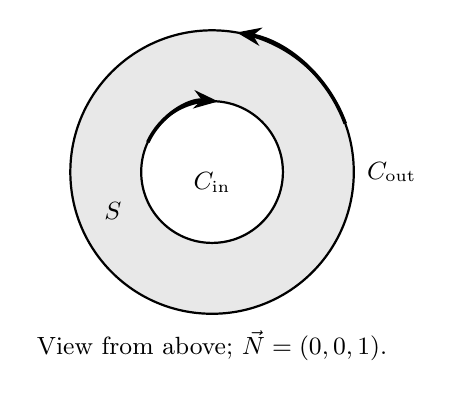
\begin{tikzpicture}[scale=0.9,>=Stealth,every node/.style={font=\small}]
\fill[gray!18,even odd rule] (0,0) circle (2) (0,0) circle (1);
\draw[thick] (0,0) circle (2);
\draw[thick] (0,0) circle (1);
\draw[->,line width=1.3pt] (20:2) arc[start angle=20,end angle=80,radius=2];
\draw[->,line width=1.3pt] (155:1) arc[start angle=155,end angle=85,radius=1];
\node[right] at (2.05,0) {$C_{\mathrm{out}}$};
\node at (0,-0.15) {$C_{\mathrm{in}}$};
\node at (-1.4,-0.55) {$S$};
\node at (0,-2.45) {View from above; $\vec N=(0,0,1)$.};
\end{tikzpicture}
\end{minipage}

\newpage

\item \textbf{Final answer:} $\boxed{3}$.

Write the plane as $z=2-2x-y$ and parametrize the sheet by
\[
\vec r(x,y)=(x,y,2-2x-y),\qquad
\left\{
\begin{aligned}
&0\le x\le1,\\
&0\le y\le2-2x.
\end{aligned}
\right.
\]
Its tangent vectors give
\[
\vec r_x=(1,0,-2),\qquad \vec r_y=(0,1,-1),\qquad
\vec n=\vec r_x\times\vec r_y=(2,1,1).
\]
The positive third component gives the required upward orientation.
The unit normal is $\vec N=(2,1,1)/\sqrt6$ and
$d\sigma=\sqrt6\,dx\,dy$, so $\vec N\,d\sigma=(2,1,1)\,dx\,dy$.

On the surface,
\[
\vec F(\vec r(x,y))=(y,x,y+2-2x-y)=(y,x,2-2x),
\]
and hence
\[
\vec F(\vec r)\cdot(\vec r_x\times\vec r_y)
=2y+x+2-2x=2+2y-x.
\]
Therefore
\[
\begin{aligned}
\iint_S\vec F\cdot\vec N\,d\sigma
&=\int_0^1\int_0^{2-2x}(2+2y-x)\,dy\,dx\\
&=\int_0^1\left[(2-x)y+y^2\right]_0^{2-2x}\,dx\\
&=\int_0^1(8-14x+6x^2)\,dx\\
&=\left[8x-7x^2+2x^3\right]_0^1=3.
\end{aligned}
\]

\bigskip
\item \textbf{Final answer:} $\boxed{6}$.

For $\vec F=(z-x^{2026},x-y^{2026},y-z^{2026})$, the curl is
\[
\operatorname{curl}\vec F
=(1-0,\ 1-0,\ 1-0)=(1,1,1).
\]
Choose the flat triangular sheet with vertices
$P=(2,0,0)$, $Q=(0,2,0)$, and $R=(0,0,2)$.
Since
\[
(Q-P)\times(R-P)=(-2,2,0)\times(-2,0,2)=(4,4,4),
\]
the stated traversal $P\to Q\to R\to P$ matches an upward normal.
Parametrize the triangle by
\[
\vec r(x,y)=(x,y,2-x-y),\qquad
\left\{
\begin{aligned}
&0\le x\le2,\\
&0\le y\le2-x.
\end{aligned}
\right.
\]
Then $\vec r_x\times\vec r_y=(1,1,1)$. By Stokes' theorem,
\[
\begin{aligned}
\oint_C\vec F\cdot\vec T\,ds
&=\iint_{S_T}(\operatorname{curl}\vec F)\cdot\vec N\,d\sigma\\
&=\int_0^2\int_0^{2-x}(1,1,1)\cdot(1,1,1)\,dy\,dx\\
&=\int_0^2\int_0^{2-x}3\,dy\,dx
=\int_0^2(6-3x)\,dx=6.
\end{aligned}
\]
The large powers disappear because only derivatives with respect to the
other components' variables enter the curl.

\end{enumerate}
\end{document}
